\subsection{Teilaufgabe 1: Algorithmik}

\subsection{Teilaufgabe 2: Theoretische Informatik}

\subsubsection{Aufgabe 1: Konstruktion}

\begin{teile}
	\item
	Sei $M = (Q, \Sigma, \delta, q_0, F)$ ein nichtdeterministischer endlicher Automat (NEA), sei $v \in \Sigma^*$ und sei $L = \{ w \in \Sigma^* \mid w \in L(M) \text{ und } w \text{ enthält } v \}$. Wir konstruieren einen NEA $M' = (Q', \Sigma, \delta', q_0', F')$, für den $L(M') = L$ gilt, wie folgt:

	\begin{itemize}
		\item $Q' = Q \times \{0, 1, \ldots, k\}$, wobei $k$ die Länge von $v$ ist.
		\item $\delta'$ ist definiert durch:
		\begin{align*}
			\delta'((q, i), \sigma) &= \begin{cases}
				\{ (q', i) \mid q' \in \delta(q, \sigma) \} & \text{falls } \sigma \neq v_{i+1}\text{ oder } i = k \\
				\{ (q', i+1) \mid q' \in \delta(q, \sigma) \} & \text{falls } \sigma = v_{i+1} \text{ und } i < k
			\end{cases}
		\end{align*}
		\item $q_0' = (q_0, 0)$
		\item $F' = \{ (q, k) \mid q \in F \}$
	\end{itemize}

	\textbf{Erklärung:}\\
	Die Zustände von $M'$ sind Paare $(q, i)$, wobei $q$ ein Zustand von $M$ ist und $i$ die Position im Wort $v$ darstellt. Wenn der Automat ein Zeichen $\sigma$ liest, das nicht das nächste erwartete Zeichen von $v$ ist, bleibt $i$ unverändert. Wenn $\sigma$ das nächste erwartete Zeichen von $v$ ist, wird $i$ inkrementiert. Sobald $i$ die Länge von $v$ erreicht hat (d.h. $i = k$), bleibt der Automat im Zustand $k$ und simuliert weiterhin $M$.

	Der Startzustand von $M'$ ist $(q_0, 0)$, und die akzeptierenden Zustände sind die Paare $(q, k)$, wobei $q$ ein akzeptierender Zustand von $M$ ist. Dies stellt sicher, dass das Wort $v$ in $w$ enthalten ist und dass $w$ von $M$ akzeptiert wird.
	
	\item
	Der Resultierende NFA sieht wie folgt aus (wobei $(q_0,1), (q_1,1)$ und $(q_2,0)$ nicht erreichbar sind und nur der Vollständigkeit des Verfahrens halber mit aufgenommen wurden):

	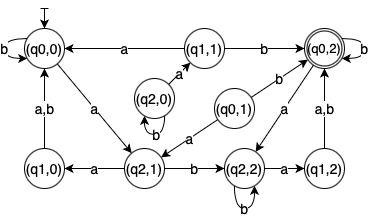
\includegraphics[scale=0.75]{NEA-Konstruktion}  
	
\end{teile}

\newpage	
\subsubsection{Aufgabe 2: Minimale DEAs}

\begin{teile}
	
	\item
		Allgemein eignet sich für die Prüfung der Minimalität eines DEA das sogenannte \glqq Tabellenfüllverfahren\grqq (im Englischen \textit{table filling algorithm} oder \textit{table filling method}). Dabei wird eine Tabelle (mit allen erreichbaren Zuständen) aufgestellt, in der nicht äquivalente Zustandspaare gekennzeichnet werden. In dieser Tabelle wird zunächst in allen Zellen, deren zugehöriges Zustandspaar einen Endzustand und einen Nicht-Endzustand enthält, ein $X_0$ notiert - diese Paare können sicher nicht äquivalent sein.\\		
		Nun wird versucht, von den übrigen Zellen aus die bereits gefüllten Zellen durch Über- gänge aus dem Automaten zu erreichen. Dies wird so lange wiederholt, bis sich keine Änderungen in der treppenförmigen Tabelle mehr ergeben. Wenn dann noch Zellen ungefüllt bleiben, bedeutet das, dass die Zustände des entsprechenden Zustandspaares äquivalent sind.\\
		Alle zueinander äquivalenten Zustände liegen dann in einer Äquivalenzklasse, die nicht äquivalenten Zustände bilden jeweils eine eigene Äquivalenzklasse. Diese Äquivalenz- klassen bilden die Zustände des minimierten DEA.
		
		Für den ersten DEA bleibt keine Zelle der Tabelle ungefüllt, was bedeutet, dass hier keine äquivalenten Zustände vorliegen. Da jeder Zustand erreichbar ist, ist der Automat also bereits minimal:
	
	\includegraphics[scale=0.75]{Tabellenfüllverfahren2.png}
	
	\begin{tabular}{c|c|c|l}
		\textbf{Zustandspaar} & \textbf{a} & \textbf{b} & \textbf{Erläuterung} \\
		\hline
		(2,1)                 & (0,1)      & (3,3)      & Eingabe b: (3,3) führt zu X0. Ergänze X1. \\
		\hline
		(2,0)                 & (0,1)      & (2,1)      & Eingabe b: (2,1) führt zu X1. Ergänze X2. \\
		\hline
		(1,0)                 & (1,1)      & (2,3)      & Eingabe b: (2,3) führt zu X0. Ergänze X3. \\
	\end{tabular} \\

	\item
		Eine Zeugentabelle zum Automaten zeigt, dass der Zustand 1 nicht erreichbar ist:

		\begin{tabular}{l|c|c|c|c}
			\textbf{Zustand} & \textbf{0} & \textbf{1} & \textbf{2} & \textbf{3} \\
			\hline
			\textbf{Zeuge} & $\epsilon$ & $-$ & $a$ & $aa$ \\
		\end{tabular}

		Die übrigen Zustände sind wieder nicht äquivalent:
	
	\includegraphics[scale=0.75]{Tabellenfüllverfahren3.png}	
	
	\begin{tabular}{c|c|c|l}
		\textbf{Zustandspaar} & \textbf{a} & \textbf{b} & \textbf{Erläuterung} \\
		\hline
		(2,0)                 & (2,3)      & (2,3)      & Eingabe b: (2,3) führt zu X0. Ergänze X1. \\
	\end{tabular}\\
	
	Der minimierte DEA sieht dann folgendermaßen aus:
	
	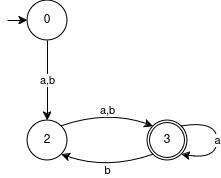
\includegraphics[scale=0.75]{MiniDEA2} 

	\item
		Für diesen Automaten bleibt nach Durchführung des beschriebenen Tabellenfüllverfahrens eine Zelle ungefüllt. Dies ist der Nachweis, dass die Zustände 1 und 3 äquivalent zueinander sind und damit in der selben Äquivalenzklasse liegen.

	\includegraphics[scale=0.75]{Tabellenfüllverfahren4.png}		
	
	\begin{tabular}{c|c|c|l}
		\textbf{Zustandspaar} & \textbf{a} & \textbf{b} & \textbf{Erläuterung} \\
		\hline
		(2,0)                 & (1,3)      & (2,3)      & Eingabe b: (2,3) führt zu X0. Ergänze X1. \\
		\hline
		(3,1)                 & (3,3)      & (1,1)      & Kein Kreuz. \\
	\end{tabular}

	Der minimierte DEA besitzt nun noch einen Endzustand und kann folgendermaßen zusammengefasst werden:
	
	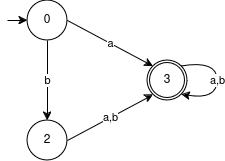
\includegraphics[scale=0.75]{MiniDEA3} 

\end{teile}

\newpage
\subsubsection{Aufgabe 3: Kontextfreie Grammatiken}

\begin{teile}
	\item
	Die Umwandlung von G in H erfolgt in vier Schritten:
 
	\textbf{1) Beseitigung von $\epsilon$-Regeln}

	Alle Regeln der Form $A \rightarrow \epsilon$ werden beseitigt. Alle Produktionsregeln, die rechts ein Nichtterminal enthalten, das zuvor zu $\epsilon$ abgeleitet werden konnte, werden dafür ergänzt um eine Kopie \textit{ohne} dieses Nichtterminalsymbol.\\
	Da das leere Wort nicht in der von H erzeugten Sprache liegen soll, muss keine weitere Regel hinzugefügt werden.

	\begin{tabular}{l|l}
		\textbf{Vorher} & \textbf{Nachher} \\
		\hline
		\begin{tabular}{lcl}
		S & $\rightarrow$ & aXY            \\
		X & $\rightarrow$ & Y $\mid$ \textcolor{red}{$\epsilon$} \\ 
		Y & $\rightarrow$ & aS $\mid$ b         \\ 
		\end{tabular} &
		\begin{tabular}{lcl}
		S  & $\rightarrow$ & aXY $\mid$ \textcolor{green}{aY}          \\
		X  & $\rightarrow$ & Y \\ 
		Y  & $\rightarrow$ & aS $\mid$ b         \\ 
		\end{tabular}
	\end{tabular}
	
	\textbf{2) Beseitigung von Kettenregeln}
	
	Jede Produktionsregel der Form A $\rightarrow$ B mit A, B $\in$ V wird als \glqq Kettenregel\grqq bezeichnet.
	Dabei werden ggf. zunächst Zykel entfernt. Da hier keine Zykel vorliegen, muss nur noch die Regel X $\rightarrow$ Y angepasst werden. Dazu wird diese Regel entfernt und alle Regeln, deren linke Seite ein Y ist, um eine neue Regel mit X als linker Seite ergänzt.
	
	\begin{tabular}{l|l}
		\textbf{Vorher} & \textbf{Nachher} \\
		\hline
		\begin{tabular}{lcl}
		S  & $\rightarrow$ & aXY                \\
		\textcolor{red}{X} & \textcolor{red}{$\rightarrow$} & \textcolor{red}{Y} \\ 
		\textcolor{blue}{Y}  & $\rightarrow$ & aS $\mid$ b         \\ 
		\end{tabular} &
		\begin{tabular}{lcl}
		S  & $\rightarrow$ & aXY                 \\
		Y  & $\rightarrow$ & aS $\mid$ b         \\
		\textcolor{green}{X}  & \textcolor{green}{$\rightarrow$} & \textcolor{green}{aS $\mid$ b}         \\ 
		\end{tabular}
	\end{tabular}
	

	\textbf{3) Ersetzen von Terminalzeichen}

	Jedes Terminalzeichen $\theta$, das in Kombination mit anderen Symbolen auftritt, wird durch ein neues Nichtterminalzeichen $\Theta$ ersetzt. Zusätzlich wird die Produktionsregel $\Theta \rightarrow \theta$ ergänzt.

	\begin{tabular}{l|l}
		\textbf{Vorher} & \textbf{Nachher} \\
		\hline
		\begin{tabular}{lcl}
			S  & $\rightarrow$ & \textcolor{blue}{a}XY                 \\
			Y  & $\rightarrow$ & \textcolor{blue}{a}S $\mid$ b         \\
			X  & $\rightarrow$ & \textcolor{blue}{a}S $\mid$ b         \\ 
		\end{tabular} &
		\begin{tabular}{lcl}
			S  & $\rightarrow$ & \textcolor{green}{A}XY                 \\
			Y  & $\rightarrow$ & \textcolor{green}{A}S $\mid$ b         \\
			X  & $\rightarrow$ & \textcolor{green}{A}S $\mid$ b         \\ 
			\textcolor{green}{A}  & \textcolor{green}{$\rightarrow$} & \textcolor{green}{a} \\
		\end{tabular}
	\end{tabular}
	
	\newpage 
	\textbf{4) Beseitigung von Nichtterminalketten} 
		
	Alle Produktionsregeln, die in der rechten Seite mehr als zwei Nichtterminalzeichen aufweisen, werden durch einfügen zusätzlicher Nichtterminale in mehrere neue Regeln mit passender Form aufgeteilt.
	
	\begin{tabular}{l|l}
		\textbf{Vorher} & \textbf{Nachher} \\
		\hline
		\begin{tabular}{lcl}
			S  & $\rightarrow$ & \textcolor{blue}{AXY} \\
			Y  & $\rightarrow$ & AS $\mid$ b         \\
			X  & $\rightarrow$ & AS $\mid$ b         \\ 
			A  & $\rightarrow$ & a \\
		\end{tabular} &
		\begin{tabular}{lcl}
			S  & $\rightarrow$ & \textcolor{green}{AZ}  \\
			\textcolor{green}{Z}  & \textcolor{green}{$\rightarrow$} & \textcolor{green}{XY} \\
			Y  & $\rightarrow$ & AS $\mid$ b         \\
			X  & $\rightarrow$ & AS $\mid$ b         \\ 
			A  & $\rightarrow$ & a \\
		\end{tabular}
	\end{tabular}
	
	Die fertige Grammatik H in CNF, für die gilt $L(H)=L(G)\backslash \{\varepsilon \}$, sieht also folgendermaßen aus:
	
	H = (V, $\Sigma$, P, S) mit V = \{S, X, Y, Z, A\}, $\Sigma$ = \{a, b\} und P:
	
	\begin{tabular}{lcl}
		S  & $\rightarrow$ & AZ  \\
		Z  & $\rightarrow$ & XY \\
		Y  & $\rightarrow$ & AS $\mid$ b \\
		X  & $\rightarrow$ & AS $\mid$ b \\ 
		A  & $\rightarrow$ & a \\
	\end{tabular} \\

	\item 
	\textbf{Erklärung} \\
	Zwei Einschränkungen gilt es zu beachten: CNF und $|V| \leq 5$. Außerdem darf die Grammatik einzig und allein das Wort \glqq aaaaaaaaaaaa\grqq\ erzeugen. \\
	Eine Nichtterminal wird benötigt, um mittels der Regel $E\rightarrow a$ letztendlich die Terminale zu erzeugen.
	Würden alle vier übrigen Variablen die Anzahl der erzeugten $a$'s mit Regeln der Form $A\rightarrow BB$ verdoppeln, würde man $2^4=16\ a$'s erhalten. Um die Anzahl zu reduzieren wird im dritten Ableitungsschritt eine Regel der Form $C\rightarrow DE$ eingebaut. So werden im vorletzten Ableitungsschritt nur die $D$'s erneut verdoppelt, während die $E$'s direkt auf Terminalsymbole abgeleitet werden. Somit werden, wie erwünscht, nur $2^3 + 2^2 = 8 + 4 = 12\ a$'s erzeugt.

	Die gesuchte Grammatik ist also $G = (V, \Sigma, P, A)$ mit $V = \{A, B, C, D, E\}$ und $P$:
	
	\begin{tabular}{lcl}
		A & $\rightarrow$ & BB \\
		B & $\rightarrow$ & CC \\
		C & $\rightarrow$ & DE \\
		D & $\rightarrow$ & EE \\
		E & $\rightarrow$ & a  \\
	\end{tabular}
	
	\item 
	------------

	TODO
	
	------------
	
	Um die Anforderung der geraden Anzahl an Terminalzeichen zu erreichen, übernehmen wir aus $P$ in $P'$ nur diejenigen Produktionsregeln, die in Ableitungsbäume abgeleitet werden können, deren Blätteranzahl geradzahlig ist. \\
	Die Einschränkung CNF bedeutet dabei, dass wir ein Nichtterminal entweder umwandeln müssen in ein Terminalzeichen, oder in zwei Nichtterminale. Es entfallen in $P'$ also alle Produktionsregeln aus $P$, die eine beliebige Verzweigung zulassen würden, wie etwa solche der Form $X \rightarrow XY | YY$.
	
\end{teile}

\subsubsection{Aufgabe 4: Berechenbarkeit}

\begin{teile}
	\item
	Ja, $L$ ist semi-entscheidbar.
	$M_1$ und $M_2$ handelt es sich um Turing-Maschinen, daher erzeugen sie Typ-0-Sprachen. \\	
	Das Wortproblem für Typ-0-Sprachen ist semi-entscheidbar.
	Auch $L$ ist eine Typ-0-Sprache, denn es ist sowohl eine Obermenge als auch eine Untermenge zweier anderer Typ-0-Sprachen. Damit ist auch $L$ semi-entscheidbar.
	
	\item
	Ja $L_1 \ L_2$ ist auch semi-entscheidbar, denn wir können eine Turing-Maschine $M'$ bauen, die $M(L_1)$ und $M(L_2)$ imitiert, und nur anhält, wenn sowohl $M(L_1)$ als auch $M(L_2)$ auf w anhalten.
	
	\item
	Ja, $L'$ ist entscheidbar, es gibt also eine Turing-Maschine M', die für jedes Wort w entscheidet, ob es zu $L'$ gehört oder nicht.

    Dafür konstruieren wir $M'(L')$ wie folgt:
	\begin{itemize}
    	\item 
    	Die Turing-Maschine erhält als Eingabe w = uv.
    	\item $M'$ prüft, ob sowohl u als auch v in $L$ gehören, indem sie die Turing-Maschine für $L$ auf beiden Teilen der Eingabe simuliert.
    	\item Falls sowohl u als auch v in $L$ sind, akzeptiert $M'$ w, andernfalls verwirft sie w.
    \end{itemize}

    Da beide Teilwörter aus der entscheidbaren Sprache $L$ stammen, wird auch $M'$ für $L'$ richtig entscheiden, ob w = uv in $L'$ liegt oder nicht. Daher ist $L'$ entscheidbar.
    
    \item
    Ja, auch $L'$ ist unentscheidbar. $L'$ besteht aus allen Präfixen von Wörtern in $L$. Wenn $L$ unentscheidbar ist, gibt es keine Möglichkeit, zu entscheiden, ob ein gegebenes Wort u zu $L'$ gehört oder nicht. Das würde nämlich bedeuten, dass wir für jedes Wort u ein entsprechendes Wort v finden müssten, so dass uv in $L$ liegt, was wiederum bedeuten würde, dass $L$ entscheidbar wäre.
	
\end{teile}